\documentclass[onecolumn,12pt]{IEEEtran}
\usepackage[margin=1in]{geometry}
\usepackage{amsfonts,amsmath}
\usepackage[affil-it]{authblk}
\usepackage{subcaption}
\usepackage{multirow}
\usepackage{algorithm}
\usepackage{algpseudocode}
\usepackage{parskip}
\usepackage[]{graphicx}
\usepackage{mathrsfs}
\usepackage{listings} 
\usepackage{color}
\usepackage{ulem}
\usepackage{hyperref}
\usepackage{booktabs}

\makeatletter
\newsavebox\zzz
\def\mystrut{%
  \dimen@\wd\zzz
  \divide\dimen@\thr@@
  \advance\dimen@-\dp\@arstrutbox
\rule\z@\dimen@}

\def\rotatezzz{ \rotatebox{90}{\rlap{\kern-\dp\@arstrutbox\usebox\zzz}}}

\makeatother
\savebox\zzz{Threads per block}

\setlength{\parindent}{1em}

\newcommand\MyHead[2]{%
  \multicolumn{1}{c}{\textbf{\parbox{#1}{\raggedleft #2}}}
}

\newcommand{\nth}{^{\text{th}}}
\title{Final Project Report}
\author{Anna Blinderman%
  \thanks{The repository for this report can be found at \href{https://github.com/blinderm/game-of-life} {\texttt{https://github.com/blinderm/game-of-life}}}}

  \author{David Kraemer}
  \author{Zachary Segall}

  \affil{CSC 213: Operating Systems and Parallel Algorithms (Curtsinger)}
  \date{May 12 2017}


  \begin{document}

  \maketitle

  \section{Project Overview}
% \begin{itemize}
%     \item introduce Game of Life
%     \item describe GUI
%     \item describe GPU stencil update
%     \item describe listener CPU threads
%     \item describe evaluation strategies
%     \item summarize evaluation results
% \end{itemize}

  We implement a variation of Conway's Game of Life -- a cellular automaton
  simulation created by the mathematician John Conway.  Scientific computing and
  large-scale simulations are incredibly useful across a variety of fields.
  However, many of these programs are prohibitively slow. Therefore the
  algorithms and design of these programs is crucial. Although Life was initially
  created as a tool to explore computability, Turing machines, and Von Neumann
  machines, the various types of optimization we explore in our project are
  applicable to a wide variety of graphics-intensive programs. 

  The Game of Life is a series of iterations of a rendering of a grid of
  cells. Each cell is either dead or alive, and there exists a simple
  deterministic algorithm that decides each cell's state at the next iteration.
  We implement a version of the Game of Life and render the simulation on an
  interactive graphical interface using the SDL framework, providing basic user
  controls such as pausing and unpausing the simulation, stepping through the 
  simulation on iteration at a time,activating and deactivating cells, and 
  clearing and quitting the application.

  For each iteration, we use Conway's algorithm to determine the state (dead or
  alive) of every cell in our grid. Because this algorithm takes as input a cell
  along with the states of each of its eight immediate neighbors, this algorithm
  naturally lends itself to an ``embarrasingly parallel" stencil computation on
  the GPU. We also have two threads running on the CPU in addition to the main
  update thread -- one for recording and acting on user input from the mouse; the
  other from the keyboard. 

  To evaluate our system, we first vary the number of threads per block in our
  stencil function calls. Then, we implement a feature that allows us to find
  regions with no live cells in order to skip their calls to the update
  functions.  We have two major findings: using the GPU significantly speeds up
  the update rate and the optimization actually slows down the update rate
  (compared to the unoptimized GPU). We hypothesize the optimization was
  ineffective because the costs of copying and extra evaluations outweigh the
  benefits of skipping some of the code.

  \section{Design and Implementation}
% \begin{itemize}
%     \item summary of overall implementation structure
%     \item Component 1: GUI
%         \begin{itemize}
%             \item responsibilities/how fits into entire structure
%             \item rationale for choice 
%             \item data structures/algorithms/libraries/other details
%         \end{itemize}
%     \item Component 2: mouse/keyboard input
%         \begin{itemize}
%             \item responsibilities/how fits into entire structure
%             \item rationale for choice 
%             \item data structures/algorithms/libraries/other details
%         \end{itemize}
%     \item Component 3: GPU stencil update
%         \begin{itemize}
%             \item responsibilities/how fits into entire structure
%             \item rationale for choice 
%             \item data structures/algorithms/libraries/other details
%         \end{itemize}
%     \item Butler Lampson's Hints for Computer System Design (integrate?)
%         \begin{itemize}
%             \item don't reinvent the wheel (+ how it did/didn't help)
%             \item be prepared to throw an entire thing out  (+ how it
%                 did/didn't help)
%         \end{itemize}
%     \item figures if appropriate
% \end{itemize}

  The rules to Conway's Game of Life are simple. There exists a grid of cells in
  which every cell is either dead or alive. At each iteration of the simulation,
  Conway's algorithm is applied to every cell in order to determine its next
  state. The algorithm\footnote{The details and history of which be found at
      \href{https://en.wikipedia.org/wiki/Conway's\_Game\_of\_Life}{\texttt{https://en.wikipedia.org/wiki/Conway's\_Game\_of\_Life}}.}
is defined in Algorithm 1.%\ref{alg:update}.

  \begin{algorithm}[t]
      \caption{How Conway's Game of Life updates the grid of cells
          Here, \textit{Grid} is a 2-dimensional array of cells, which all have
          a \textit{state} field. Two cells are neighbors if they are adjacent
      in the 2-dimensional array.}
      \begin{algorithmic}
          \Function{update\_grid}{\textit{Grid}} 
          \For {$g \in \textit{Grid}$}
          \State $N(g) \gets \{ h \in \textit{Grid} : \textrm{$h$ is a neighbor
          of $g$}\}$
          \State $s \gets \sum_{h \in N(g)} h.\textit{state}$
          \If {$s < 2$ or $s > 3$}
          \State $g.\textit{state} \gets 0$
          \Else
          \If {$s = 2$ and $g.\textit{state} = 0$}
          \State $g.\textit{state} \gets 0$
          \Else 
          \State $g.\textit{state} \gets 1$
          \EndIf
          \EndIf
          \EndFor
          \EndFunction
      \end{algorithmic}
      \label{alg:update}
  \end{algorithm}

  With these baseline rules, we implement a system in which the user is able to
  click cells to switch their state, pause and run the simulation
  automatically, or step through various iterations. We also have features that
  go beyond the basic simulation, including reading boards from files, adding
  gilders to the board, and having cells change color as the age. The exact
  specifications for adjustable features are as follows:

  \begin{itemize}
    \item GUI (game board) display size
    \item cell size (thus adjusting the number of cells) 
    \item delay between iterations while running simulation
    \item colors, including linear interpolation between start and end values
    \item can randomize a board
    \item can load board from file
  \end{itemize} 
  During the simulation, the user's options are provided in Table
  \ref{tab:gui}.
  \begin{table}[t]
    \centering
    \begin{tabular}[b]{@{}lp{10cm}@{}} \toprule
      Input & Behavior \\ \midrule
      Left click (or drag) & Toggle the cell enclosing the current mouse
      pointer's location to ``alive.'' \\
      Right click (or drag) & Toggle the cell enclosing the current mouse
      pointer's location to ``dead.'' \\
      Press \texttt{CTRL-Q} & Quits the simulation and closes the GUI. \\
      Press \texttt{CTRL-C} & Clears the simulation game board. \\
      Press \texttt{CTRL-P} & (Un)pauses the simulation. \\
      Press \texttt{CTRL-SPACE} & Advances the simulation by one step (while
      paused). \\
      Press \texttt{CTRL-G} & Populates the region around the mouse's current
      location with a glider. \\ \bottomrule
    \end{tabular}
    \caption{User input options together with the resulting behavior.}
    \label{tab:gui}
  \end{table}
  Given that the update algorithm is itself simple to implement, most of our
  difficulties were centered around coordinating between the GUI display, the 
  user input CPU threads, and the update algorithm on the GPU.	

  We start development with the GUI, which is responsible for displaying the
  board and updates with reasonable response time. We use the bitmap class from
  the Galaxies lab for the GUI because it offers high resolution for the display
  and easily adjustable parametes. Reusing the bitmap also follows Lampson's
  principle of ``reuse good ideas" - we already have a class built for exactly
  what we want to do, so there's no need to reinvent the wheel. The GUI itself
  gave us no difficulties in our implementation. 

  Although both the bitmap class and The Game of Life are represented with grids,
  the bitmap provides a much higher resolution of squares than we wish to use
  for the representation of cells on the grid. Thus there are two options: use
  the bitmap and have multiple pixels refer to the same cell, or have a separate
  struct for the grid and translate between the grid struct and the bitmap. We
  opt for the latter. This separation allows us to more easily manipulate and
  update the representation and then simply update the visualization afterwards
  using Conway's original algorithm. The cells on the game board are initially 
  populated from either a random starting configuration, one of some set of
  preset starting configurations, or by the user clicking squares on the board. 

  To handle user input, we intended to use a scheduler (as in the Worm lab) in
  order to split up listening for input and updating across processes. We quickly
  ran into problems with this approach, as the listeners would sometimes fail to
  register input if they weren't being executed by the scheduler at the exact
  moment the user clicked or pressed a button. Thus, we realized we needed
  complete concurrency on the CPU and switched to an implementation with threads:
  one for mouse input, one for keyboard input, and the main one to run updates.
  At this point, we applied Lampson's lesson of ``Throw one away" and gave up on
  our scheduler-based approach. As we will discuss later, our listener threads 
  handle user input perfectly. This switch from the scheduler to the listener
  threads on the CPU was integral in our building a working program.

  In order for the threads to properly take in and act on user input, we have a
  struct which contains the information necessary for the various actions in the
  program to be taken -- the location of the cell from which the user input was
  recorded, the state of the mouse (clicked or unclicked), and the
  \texttt{SDL\_Event} which indicates the state of the user input devices to SDL.
  The mouse thread is then responsible for executing the first two of the above
  bullet points when appropriate; the keyboard thread is responsible for the
  other five. The main thread calls our update function. In any case, this struct
  of arguments is passed to the functions so that they may act appropriately. 

  We use SDL to register user input from both the mouse and the keyboard. Any
  mouseclick or button-presstriggers an update to the main \texttt{SDL\_Event},
  which is then sent to the mouse and keyboard event handler loops. Mouse events
  are handled by checking that the mouse state generated from
  \texttt{SDL\_GetMouseState} on the current location is one of
  \texttt{SDL\_BUTTON\_LEFT} or \texttt{SDL\_BUTTON\_RIGHT}. A left press turns
  the cell in which the mouse event is located to ``alive,'' and a right press
  turns the cell to ``dead.'' Pressing down the left mouse button triggers the
  simulation to toggle the cell in which the mouse pointer is located to
  ``alive,'' and similarly, pressing down the right mouse button triggers the
  simulation to toggle the cell to ``dead.'' This feature allows the user to
  ``click and drag'' to toggle a series of adjacent cells.

  Keyboard events are handled so that a full button press and release are
  required before the command is executed in the simulation. Upon receiving a new
  \texttt{SDL\_Event}, the keyboard handler thread checks if the event type is
  \texttt{SDL\_KEYDOWN} or \texttt{SDL\_KEYUP}. If the type is
  \texttt{SDL\_KEYDOWN} on a pre-specified command key, then a ``tripwire'' is
  set. If the type is \texttt{SDL\_KEYUP} and the ``tripwire'' is active, then
  the command is executed. This feature prevents anything analogous to the
  ``click and drag'' from occurring with key presses.  For the simulation itself to run, we must update all cells in our board
  according to Conway's original algorithm. As described above, this algorithm
  naturally lends itself to an ``embarrassingly parallel" implementation. The
  update function progresses in two steps: first, we used a stencil pattern since
  a cell's next state depends on the states of its eight immediate neighbors,
  then use a map pattern to process whether or not a cell survives. We actually
  have two grids in the program: one that stores counts each cell's neighbors and
  one that stores the actual age of each cell. The steps are parallelizable
  because the state of a cell depends only on the states of the cells in the past
  iteration (i.e. not on any of the states of the other updated cells). Between
  each call of the update function, we copy the grid between the GPU and the CPU
  in order to account for user input.

  \section{Evaluation}

  \begin{figure}[t]
    \centering
      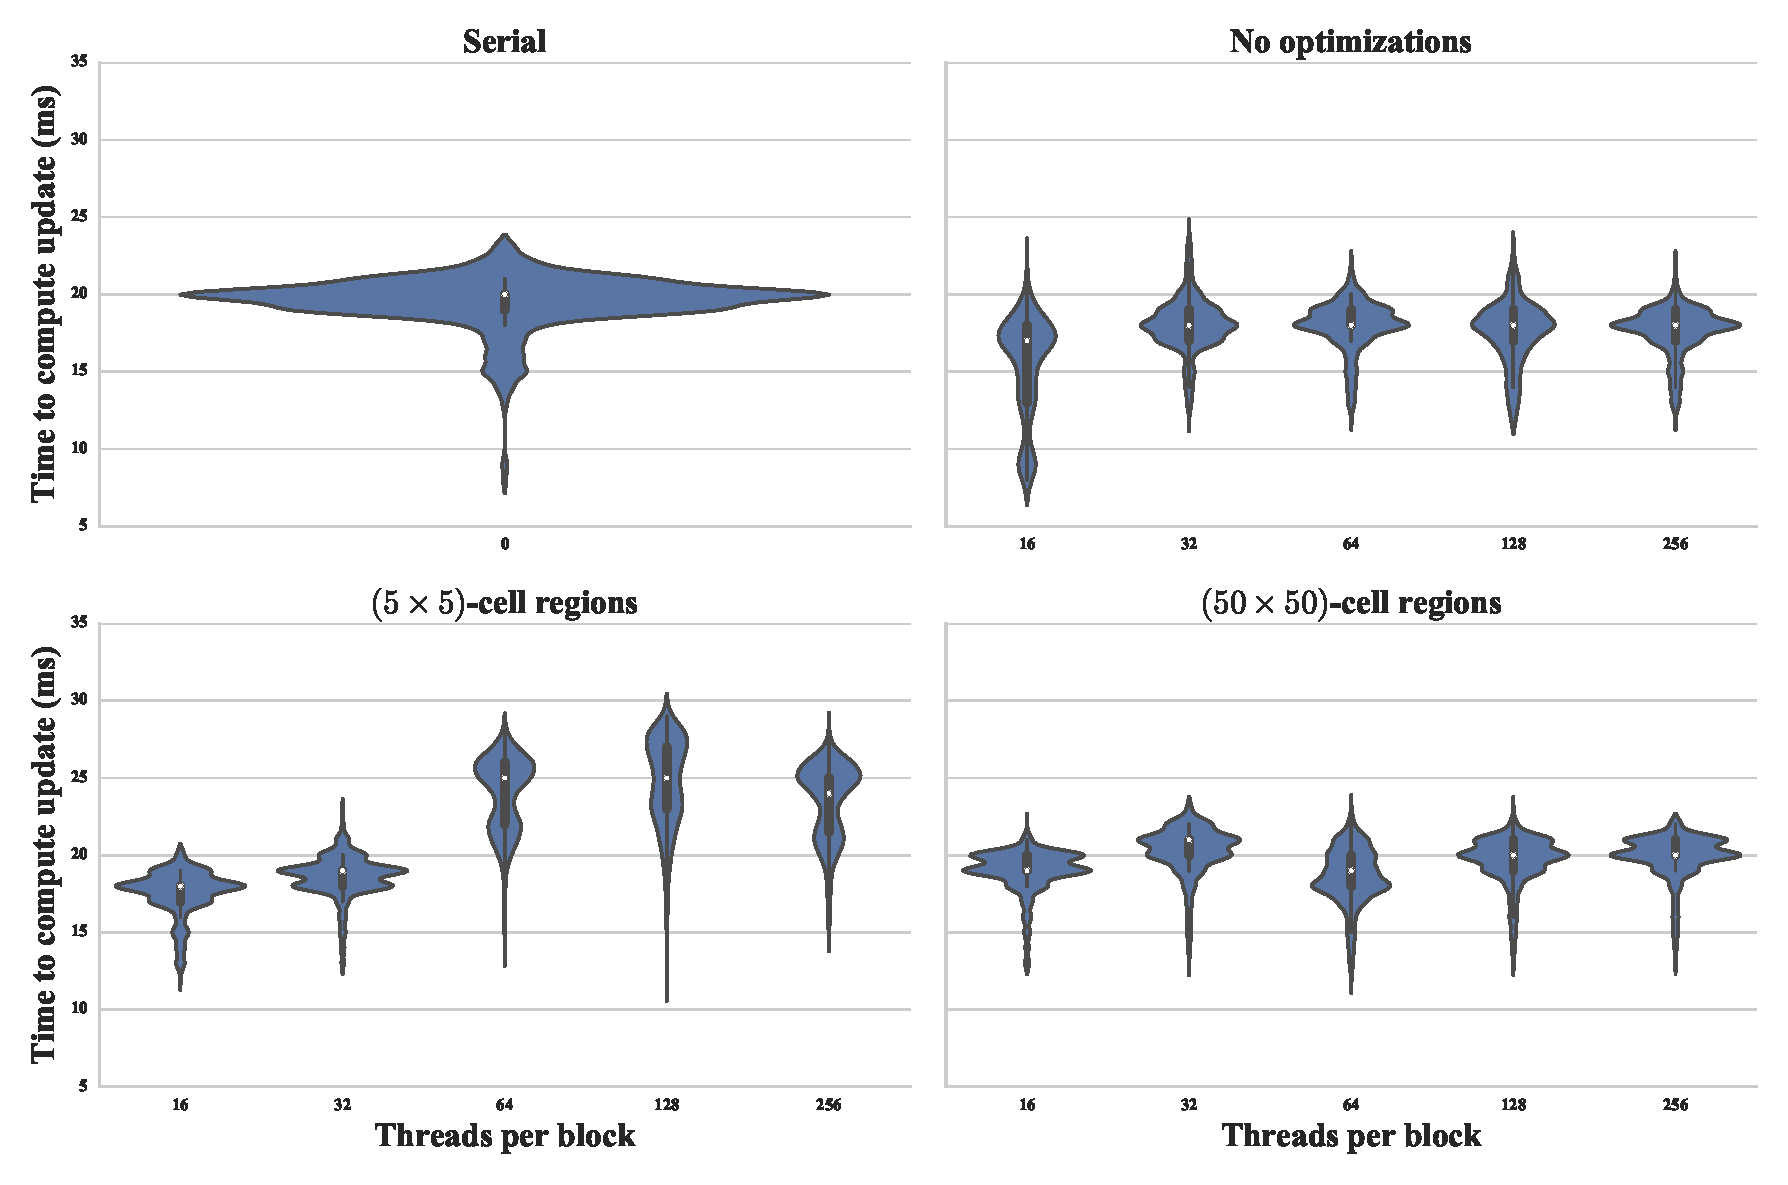
\includegraphics[width=\textwidth]{../images/boxplot.eps}
    \caption{Distribution of Update Times by Threads Per Block (T/B) and Optimization Region Dimension conditions}
    \label{fig:boxplots}
  \end{figure}

  \begin{figure}[t]
    \centering
    \begin{subfigure}[t]{0.6\textwidth}
    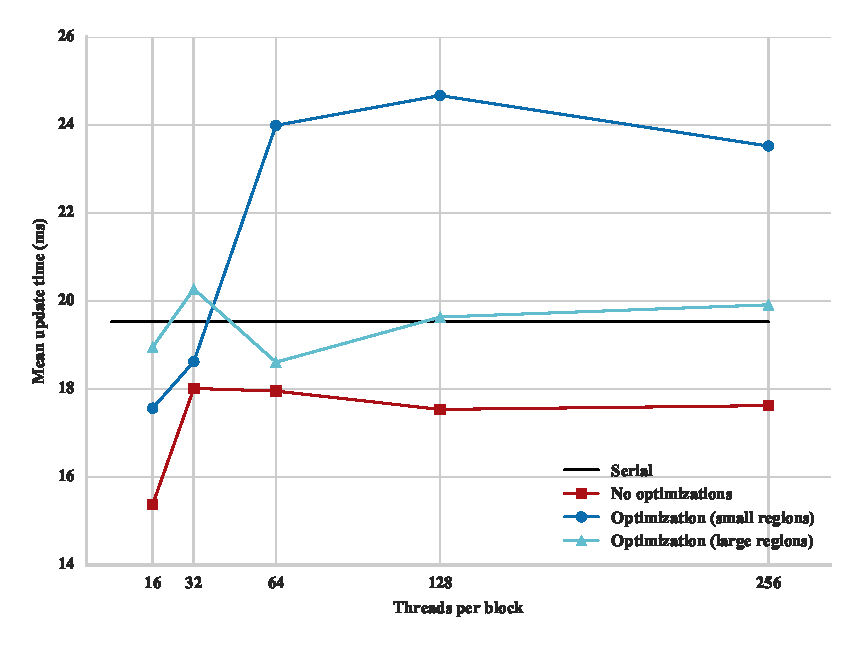
\includegraphics[width=0.9\textwidth]{../images/plot.eps}
      \caption{Comparing Mean Update Time (ms) to Thread Per Block (T/B)}
      \label{fig:comparison}  
    \end{subfigure}
    \begin{subfigure}[t]{0.3\textwidth}
      \centering
      \begin{tabular}[b]{@{}*{4}{r}@{}} \toprule
          \multirow{2}{*}{T/B} 
          & \multicolumn{3}{c}{Region Dimension} \\
                           & 0        & 5       & 50 \\ \midrule 
          Serial           &  19.514  &  N/A    & NA \\
          16               &  15.402  &  17.589 &  18.981 \\
          32               &  18.040  &  18.646 &  20.290 \\
          64               &  17.963  &  24.019 &  18.633 \\
          128              &  17.565  &  24.675 &  19.660 \\
          256              &  17.644  &  23.528 & 19.919 \\ \bottomrule
      \end{tabular}
      \caption{Mean Update Time (ms) by Threads Per Block (T/B) and Optimization Region Dimension}
      \label{tab:means}
    \end{subfigure}

  \end{figure}


% \begin{itemize}
%     \item describe experimental setup (Anna)
%         \begin{itemize}
%             \item hardware (???)
%             \item software (libraries)
%             \item data-gathering methods (Anna)
%         \end{itemize}
%     \item explain what trying to measure (speedup)  (Anna)
%         \begin{itemize}
%             \item vary block size
%             \item implement thing that only updates regions with living things?
%             \item implement serial version?
%         \end{itemize}
%     \item include at least one graph with at least 8 data points [friend]
%     \item discuss interpretation of results [friend]	
% \end{itemize}

  The hardware needed to run our evaluations is the same as that which is needed
  to run our program in general: a computer with an Nvidia GPU and SDL. For our
  statistical analysis and production of graphs, we use \texttt{Python},
  specifically with the \texttt{pandas} library to hold our data, the
  \texttt{numpy} package to run our analyses, and the \texttt{matplotlib} library
  to produce our figures.  

  In addition to ensuring that our implementation properly reflects Conway's
  rules, we verify that the concurrent components of our system function
  properly. For our listener threads on the CPU, we notice from running many
  tests that the program's response to user input is both immediate and correct. 

  However, the speed of our program is our main focus in our evaluations. As a
  benchmark, we implement a serial version of each of our GPU kernel functions
  involved in the advancement of our simulation from one iteration to the next.
  In order to test the efficiency of our parallelized program against that of the
  serial version, we create a file and use \texttt{time\_ms} to measure the
  running time of our update function and write that information to the file. 

  For our serial implementation, we loop over every cell in our grid to count the
  number of its neighbors that are alive. Then we apply Conway's algorithm to
  decide what its state will be at the next iteration. Finally, we loop over each
  pixel in our bitmap in order to correctly render these updates to the screen.
  Our parallel implementation is similar, although we count neighbors and update
  our cell grid using blocks of threads. 

  We run 1000 iterations of our serially-implemented simulation and collect the
  running time of each of the 1000 updates in a file. We do five similar runs
  for our parallel implementation, testing threads per block values of 16, 32,
  64, 128, and 256.

  Before proceeding to the experimental analysis, we remove a consistent outlier
  from the results of each configuration, which was always the first update.
  There is likely additional startup costs to the initial GPU setup which is
  captured in the first run of the update, which is true across each
  configuration. We perform a statistical test to decide the significance in the
  mean time to update between any two configurations. Since the populations
  appear to be, very roughly, approxmating a normal distribution, and because we
  have no prior information about the parameters of the distribution of the
  configuration we are sampling from, the 2-sample $t$-test is the appropriate
  statistical test. Our significance level is taken to be $\alpha = 0.01$. There
  are 128 such tests, the vast majority of which yield significant results. We
  record the insignificant results in Table \ref{tab:stats}. For example, there
  is no significant difference between the configuration with small regions and
  16 threads per block, and either configurations with no optimizations and 128
  and 256 threads per block.  This is evident in Figure \ref{fig:comparison}. The
  sample distributions from each configuration are displayed in Figure
  \ref{fig:boxplots}.

  While running our simulations, we noticed a possible way to speed up our code
  further: because there are oftentimes large regions of the board in which there
  are no live cells, we can know that there is no need to check for updates in
  such regions. Thus, running the kernel function on those cells is
  computationally wasteful. In order to reduce the effects of this inefficiency,
  we overlay yet another grid onto our board. This ``regions" grid, which is of
  lower dimension than our grid of cells, holds the a count of the number of live
  cells within its boundaries. We then modify our GPU kernels so that they only
  run the main body on cells that are in regions with at least one live cell. We
  again run 1000 iterations of this program, testing all ten combinations of the
  five threads per block values from above and a ``region" dimension of either 5
  or 50. In our current implementation, we ignore edge cases for simplicity
  (within a region, we must actually check the entirety of the region as well as
  another layer of cells surrounding it in order to ensure no cell within the
  region will be updated), so these tests report a lower runtime for our
  optimized runs than they would if our optimization were implemented completely.
  For the resulting means, see Table \ref{tab:means} and Figure \ref{fig:comparison}.
  
  Our experiment shows that there is a negligible speedup in performing the
  region optimization. In fact, by comparing the mean update time in Table
  \ref{tab:means}, we observe that the optimizations actually worsen the overall
  performance of the simulations. Copying from the CPU to the GPU and vice versa
  is the likeliest cause for the added cost to the performance of the
  optimizations. The basic data model has an SDL bitmap and a lower-resolution
  game board which is represented on both the CPU and GPU.  Both optimizations
  add an additional board which is again represented on both the CPU and GPU. 
  The improvements in performance by ignoring inactive regions are more than 
  offset by the memory copying between the CPU and GPU.

  There is essentially no improvement in performance as the number of threads per
  block increases. This is likely because the total number of active threads
  running on the GPU does not change as the number of threads per block
  increases. Since the Game of Life update algorithm is an embarassingly parallel
  problem, there is likely no added benefit to the changing the structure of each
  block. This does not explain the apparent speed penalty for small regions
  incurred for 64, 128, and 256 threads per block (see Figure
  \ref{fig:boxplots}), which doesn't yield a simple interpretation.
  
  Thus, we see that our parallelization of Conway's algorithm using GPU kernels
  is the optimization feature that consistently improves our program's
  efficiency.

  \begin{table}
    \centering
    \caption{Statistically insignificant 2-sample $t$-test results ($p = 0.01$).}
    \begin{tabular}{rrrrrr} \toprule
      \multicolumn{2}{c}{\textbf{Configuration A}} &
      \multicolumn{2}{c}{\textbf{Configuration B}}
      \\
      Region Dimension & Threads/block &  Region Dimension & Threads/block &
      $t$-statistic & $p$-value \\ \midrule
      5  & 16  &      0 &   128  & -0.274335 & 0.783856 \\
      5  & 16  &      0 &   256  &  0.735564 & 0.462082 \\
      0  & 32  &      0 &    64  & -0.969775 & 0.332276 \\
      5  & 32  &     50 &    64  & -0.165566 & 0.868515 \\
      0  & 128 &      0 &   256  &  0.892050 & 0.372473 \\
      50 & 128 & Serial & Serial & -1.870520 & 0.061558 \\ \bottomrule
    \end{tabular}
    \label{tab:stats}
  \end{table}

  \end{document}
